\chapter{MARCO TEÓRICO}
\section{MARCO CONCEPTUAL}
\subsection{LeapMotion}
.
\subsection{Goniometria}
.
\subsection{Análisis de puesto de trabajo}
.
\subsection{Enfermedades y lesiones}
 Un Desorden Músculo Esquelético (DME) es una lesión física originada por trauma acumulado que se desarrolla gradualmente sobre un período de tiempo; como resultado de repetidos esfuerzos sobre una parte específica del sistema músculo esquelético. \footcite[]{MinisterioQue}. A continuación se presentan las enfermedades prevalentes en los puestos de trabajo para manos, muñeca y antebrazo

\subsubsection{Tenosinovitis De Quervain}
\paragraph{¿Qué es?}
La Tenosinovitis De Quervainn (TDQ) también conocida como tenosinovitis estiloides radiales, consiste en la inflamación de los tendones del pulgar a causa de movimientos repetitivos.

\begin{figure}[H]
    \centering
    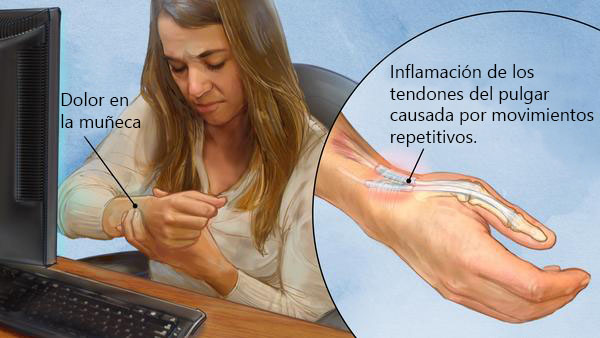
\includegraphics[width=0.7\textwidth]{Anexos/LATEX/chapters/images/TDQ.jpg}
    \caption{Anatomía de la mano con TDQ \\\textbf{Fuente:} https://g.co/kgs/BpkB4A}
    \label{TDQ}
\end{figure}

Esta enfermedad se manifiesta como una inflamación que produce una estenosis del canal osteofibrososinovial situado en la estiloides radial por el que discurren los tendones del abductor largo y extensor corto del pulgar. Se produce al combinar agarres con giros o desviaciones cubitales y radiales repetidas o forzadas de la mano.\footcite[2]{TenosinovitisDelPulgarDDCENFERMEDADESTME}

De acuerdo al Instituto Nacional de Seguridad e Higiene en el Trabajo de España, la Enfermedad de Quervain (CIE-9 MC 727.04) posee un tiempo estándar de incapacidad temporal de 20 días.\footcite[6]{TenosinovitisDelPulgarDDCENFERMEDADESTME}
\paragraph{Prevención}
Se aconseja no combinar agarres con giros o desviaciones cubitales y radiales repetidas. Para las situaciones de oficina que involucran un mouse, es necesario evitar realizar desplazamientos girando la muñeca, el movimiento adecuado debe ser desplazar el brazo en su totalidad desde el hombro
\subsubsection{Síndrome del Túnel del Carpo}
\paragraph{¿Qué es?}
Existe un espacio en la muñeca llamado túnel del carpo, a través del cual pasan el nervio mediano y nueve tendones flexores que van desde el antebrazo hacia la mano. El Síndrome del Túnel del Carpo (STC) es una condición producida por la compresión del Nervio Mediano, a nivel de la muñeca. Esta compresión produce entumecimiento, hormigueo y dolor en la mano, dedos y ocasionalmente en el brazo. \footcite{SindromeCarpiano}

\begin{figure}[H]
    \centering
    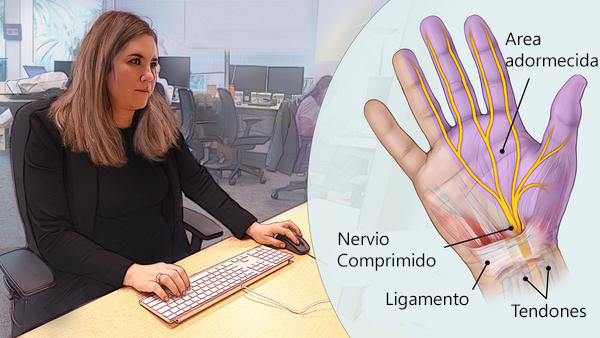
\includegraphics[width=0.7\textwidth]{Anexos/LATEX/chapters/images/STC.jpg}
    \caption{Anatomía de la mano con STC \\\textbf{Fuente:} https://g.co/kgs/MdPBTe}
    \label{STC}
\end{figure}

El STC se presenta cuando se aumenta la presión dentro del túnel por cualquier proceso inflamatorio, comprimiendo el nervio, el cual es una estructura muy sensible a los aumentos de presión. Cuando la presión dentro del túnel es muy alta y altera la función normal del nervio, aparecen rigidez, hormigueo y dolor en la mano y los dedos.\footcite{SindromeCarpiano}
\paragraph{Prevención}
Es recomendable informar al trabajador, entrenándolo para que aquellas posturas o movimientos peligrosos sean evitados durante el desarrollo de su labor, además, el buen diseño de las herramientas, utensilios y del puesto de trabajo ayudan a conseguir la relajación de la mano y de la muñeca.\footcite{SindromeTratarlo}

\subsubsection{Síndrome del túnel cubital}
%http://www.insht.es/InshtWeb/Contenidos/Documentacion/FICHAS%20DE%20PUBLICACIONES/EN%20CATALOGO/ERGONOMIA/Ficha6epitrocleoolecranian.pdf
\subsection{Legislación Vigente}
\section{MARCO REFERENCIAL}
\subsection{Modelos de valoración del riesgo contexto nacional}
\subsubsection{Normas GATI-SO}
Las Guías de Atención Integral de Salud Ocupacional Basadas en la Evidencia (GATI-SO) nacen a partir de un plan de trabajo propuesto por la dirección general de riesgos profesionales del ministerio de la protección social con el objetivo de incrementar el diagnóstico y prevenir las enfermedades profesionales de
mayor prevalencia en Colombia.\footcite[6]{MinisterioQue}

Las características de los factores de riesgo ocupacional que han demostrado estar asociados con la aparición del \textbf{STC} son las siguientes:\footcite[45]{MinisterioQue}
\begin{itemize}
\item Posturas en flexión y extensión de dedos, mano y muñeca, así como, la desviación ulnar o radial que implique agarre, pronación y supinación combinada con el movimiento repetitivo en ciclos de trabajo
\item Fuerza ejercida en trabajo dinámico por manipulación de pesos en extensión y flexión de los dedos y la mano
\item Vibración segmentaría derivada del uso de herramientas vibratorias
\end{itemize}
Las características de los factores de riesgo ocupacional que han demostrado estar asociados con la aparición del \textbf{TDQ} son las siguientes:\footcite[45]{MinisterioQue}
\begin{itemize}
\item Postura forzada de muñeca asociada a movimiento de alta repetición (ciclos de tiempo menores a 30 segundos o 50 \% del ciclo gastado.
\end{itemize}
Adicionalmente se mencionan las siguientes conclusiones:\footcite[46]{MinisterioQue}
\begin{itemize}
\item Existe evidencia de que las posturas asumidas de codo, antebrazo y mano se asocian con mayor frecuencia a los desórdenes de trauma acumulativo en población trabajadora.
\item Existe evidencia de que el movimiento repetitivo se asocia con mayor frecuencia a los desórdenes de trauma acumulativo en población trabajadora.
\item Existe evidencia de que la fuerza se asocia con mayor frecuencia a los desórdenes de trauma acumulativo en población trabajadora.
\end{itemize}



\section{Métodos de evaluación de posturas}
El factor de riesgo que más se relaciona a la aparición de DME se conoce como carga postural. Cuando se llevan a cabo posturas inadecuadas a manera continua o repetitiva se genera fatiga, la cual con el tiempo puede ocasionar problemas de salud. Por lo tanto, la medición de la carga postural constituye el pilar principal en el proceso de mejora de puestos de trabajo.\footcite[144]{RamosEdgarShrawan2004WorkingReview}
\subsection{Método Rula}
El método RULA tiene como objetivo de evaluar la exposición de los trabajadores a factores de riesgo que originan una elevada carga postural y que pueden ocasionar trastornos en los miembros superiores del cuerpo. Para la evaluación del riesgo se consideran el método la postura adoptada, la duración, la frecuencia y las fuerzas ejercidas cuando se mantiene.\footcite[2]{McatamneyRULA:Disorders}

Para una determinada postura RULA obtendrá una puntuación a partir de la cual se establece un determinado Nivel de Actuación. El Nivel de Actuación indicará si la postura es aceptable o en qué medida son necesarios cambios o rediseños en el puesto. En definitiva, RULA permite al evaluador detectar posibles problemas ergonómicos derivados de una excesiva carga postural.\footcite{Diego-Mas2015EvaluacionRULA}.

RULA divide el cuerpo en dos grupos, el Grupo A que incluye los miembros superiores (brazos, antebrazos y muñecas) y el Grupo B, que comprende las piernas, el tronco y el cuello. Mediante las tablas asociadas al método, se asigna una puntuación a cada zona corporal (piernas, muñecas, brazos, tronco...) para, en función de dichas puntuaciones, asignar valores globales a cada uno de los grupos A y B
\subsection{Método Reba}
\subsection{Método Owas}
\subsection{Evaluación Postural Rápida}
\subsubsection{}
\section{MARCO TECNOLÓGICO}